% \RequirePackage[l2tabu, orthodox]{nag}
%% Checks for obsolete LaTeX packages and outdated commands. 
%% Does nothing as long as your syntax is right.

\documentclass[12pt]{amsart}




% Document class possibilities:
%   amsart, article, book, beamer, report, letter
% Options:
%   letterpaper, a4paper,11pt,oneside, twoside, draft, twocolumn, landscape

%% For beamer class, see my beamer template.

%% ========== Options to Toggle When Compiling ==============
%\usepackage{syntonly}
%\syntaxonly


%%%%%%% Show Keys %%%%%%%%%%%%%%%%%%%
%\usepackage[notcite]{showkeys} 

%%%%%%%%%%%%%%%%%%%%%%%%%%%%%%%%%%

%% Show tags and labels.
% %\usepackage{layout}            %% Show variable values controlling page layout.
%\allowdisplaybreaks[1]         %% Allow multiline displays to split.
%\nobibliography     %% Use proper citations, but do not generate bibliography.

%% ========== Select *.tex file encoding and language ==============
%\usepackage[language]{babel} %% Takes care of all language requirements.

%\usepackage[latin1]{inputenc}  %% Use with PuTTY or TeXMaker
%\usepackage[utf8]{inputenc}  %% Use on most OS's, such as Ubuntu.

%% ============== Page Styles ==============
 \usepackage{fancyhdr}
% \pagestyle{fancy}
% \pagestyle{empty}

%% ============== Page Layout ==============
%% Allow extra space at the bottom of pages.
% \raggedbottom     

%% Use smaller margins.
%\usepackage{fullpage}

%%Control page number placement.  \thepage is the current page number.
% \renewcommand{\headrulewidth}{0pt}
% \lhead{}
% \chead{}
% \rhead{}
% \lfoot{}
% \cfoot{\thepage}
% \rfoot{}

\usepackage[margin=1in]{geometry}  %% Can adjust the margins of individual pages
\usepackage{setspace}
\usepackage{caption}
\usepackage{siunitx}
%% Use it like this:
%% \newgeometry{left=3cm,bottom=0.1cm}
%%     ... Lines that require margins adjusted ...
%% \restoregeometry

%% ============== Math Packages ==============
\usepackage{amsmath}
\usepackage{amsfonts}
\usepackage{amssymb}
\usepackage{amsthm}
\usepackage{mathtools} % An improvement of amsmath
\usepackage{latexsym}

%% ============ Typesetting add-ons ============
%\usepackage{siunitx} %Support for SI units, \num, \SI, etc.

%% ============== Single-Use Packages ==============
\usepackage{enumerate}
\usepackage{cancel}
\usepackage{cases}
\usepackage{empheq}
\usepackage{multicol}

%% ============== Graphics Packages ==============
\usepackage{graphicx} %% Conflicts with pdflatex.
%\usepackage{graphics} %% Conflicts with eps files.
%\usepackage{epsfig} Allows eps files (?)

\usepackage{wrapfig}

%% Note: For using .eps graphics, use the graphicx package,
%% and in the document use, for example:
%% \begin{figure}
%%  \includegraphics[scale=0.5]{my_picture.eps}
%% \end{figure}

%% Prevent figures from appearing on a page by themselves:
%\renewcommand{\topfraction}{0.85}
%\renewcommand{\textfraction}{0.1}
%\renewcommand{\floatpagefraction}{0.75}

%% Force floats to always appear after their definition: 
%\usepackage{flafter}

%% ============== tikZ and PGF packages ==============
%\usepackage{ltxtable,tabularx,tabulary}
 
% \usepackage{tikz}
% \usepackage{pgf}
% \usepackage{pgfplots} %% Requires pgf 2.0 or later.
% % \usetikzlibrary{arrows, automata, backgrounds, calendar, 
% % chains,matrix, mindmap, patterns, petri, shadows, 
% % shapes.geometric,shapes.misc,
% % spy, trees}
% \pgfplotsset{compat=1.9} % Fixes some backwards compatibility warnings
% \usetikzlibrary{arrows}

%% ============== Colors ==============
%% Warning: These are often a source of conflicts during compilation.
\usepackage{color}
\newcommand{\blue}[1]{{\color{blue} #1}}
\newcommand{\red}[1]{{\color{red} #1}}

%% ============== Notes ==============
\usepackage[color=white,linecolor=black]{todonotes}
% \usepackage[backgroundcolor=gray!30,linecolor=black]{todonotes}
% \usepackage[disable]{todonotes}
%\listoftodos, \todo[noline]{}, \todo[inline]{}, \todo{}, \missingfigure{}
% \todo]{}
   
%% ============== Fonts ==============
%\usepackage{bbm}  %% Non-Vanilla: Not include in many LaTeX distributions.
\usepackage{mathrsfs}
\usepackage{fontenc} %T1 font encoding
\usepackage{inputenc} %UTF-8 support
%\usepackage{babel} %Language specific commands, shortcuts, hyphenation.

\usepackage{verbatim}

%% Microtype improves spacing.  Load after fonts.
% \usepackage{microtype}

%% ============== Theorem Styles ==============
%% Note: newtheorem* prevents numbering.

\theoremstyle{plain}
\newtheorem{theorem}{Theorem}[section]
\newtheorem{proposition}[theorem]{Proposition}
\newtheorem{lemma}[theorem]{Lemma}
\newtheorem{corollary}[theorem]{Corollary}
\newtheorem*{claim}{Claim}

\theoremstyle{definition}
\newtheorem{definition}[theorem]{Definition}
\newtheorem{example}[theorem]{Example}
\newtheorem{exercise}[theorem]{Exercise}
\newtheorem{axiom}[theorem]{Axiom}

\theoremstyle{remark}
\newtheorem{remark}[theorem]{Remark}

%% ============== References ==============
\setcounter{secnumdepth}{3} %% Used to label subsections
\numberwithin{equation}{section} %% Equation numbering control.
\numberwithin{figure}{section}   %% Figure numbering control.

\usepackage[square,comma,numbers,sort]{natbib}
\usepackage[colorlinks=true, pdfborder={ 00 0}]{hyperref}
\hypersetup{urlcolor=blue, citecolor=red}
\usepackage{url}

%% Reference things as 'fig. 1', 'Lemma 7', etc.
\usepackage{cleveref}

%% Create references like 'on the following page', 'on page 23'
% \usepackage{varioref} 

% usepackage[refpages]{gloss} %% Glossary

%%%%%%%%%%%%%%%%%%%%% MACROS %%%%%%%%%%%%%%%%%%%%%

% ============================== Vectors ==============================
\newcommand{\vect}[1]{\mathbf{#1}}
\newcommand{\bi}{\vect{i}}
\newcommand{\bj}{\vect{j}}
\newcommand{\bk}{\vect{k}}

\newcommand{\bn}{\vect{n}}

\newcommand{\bu}{\vect{u}}
\newcommand{\bv}{\vect{v}}
\newcommand{\bw}{\vect{w}}
\newcommand{\boldm}{\vect{m}}
\newcommand{\bx}{\vect{x}}
\newcommand{\by}{\vect{y}}
\newcommand{\bz}{\vect{z}}

\newcommand{\be}{\vect{e}}
\newcommand{\bg}{\vect{g}}

\newcommand{\bbf}{\vect{f}}

% ==================== Fields ==================
\newcommand{\field}[1]{\mathbb{#1}}
\newcommand{\nN}{\field{N}}
\newcommand{\nZ}{\field{Z}}
\newcommand{\nQ}{\field{Q}}
\newcommand{\nR}{\field{R}}
\newcommand{\nC}{\field{C}}
\newcommand{\nF}{\field{F}}
\newcommand{\nK}{\field{K}}

% ======================== Script Symbols  ========================
\newcommand{\sL}{\mathscr L}
\newcommand{\sH}{\mathscr H}
\newcommand{\sG}{\mathscr G}

% ====================== Caligraphic Symbols ======================
\newcommand{\cA}{\mathcal A}
\newcommand{\cB}{\mathcal B}
\newcommand{\cC}{\mathcal C}
\newcommand{\cD}{\mathcal D}
\newcommand{\cF}{\mathcal F}
\newcommand{\cH}{\mathcal H}

\newcommand{\cK}{\mathcal K}
\newcommand{\cL}{\mathcal L}

% ======================== Fraktur Symbols  ========================
% Note: Use mathrsfs package.

\newcommand{\fm}{\mathfrak m}

% ========================== Bold Symbols ==========================
\newcommand{\bvphi}{\boldsymbol{\vphi}}
\newcommand{\bPhi}{\boldsymbol{\Phi}}

% ======================== Misc. Symbols ========================
\newcommand{\nT}{\mathbb T}
\newcommand{\vphi}{\varphi}
\newcommand{\maps}{\rightarrow}
\newcommand{\Maps}{\longrightarrow}
\newcommand{\sand}{\quad\text{and}\quad}
\newcommand{\QED}{\hfill$\blacksquare$}
\newcommand{\tac}{\textasteriskcentered}
%\newcommand{\dhr}{\m\athrel{\lhook\joinrel\relbar\kern-.8ex\joinrel\lhook\joinrel\rightarrow}}

% ========================== Operations ==========================
\newcommand{\cnj}[1]{\overline{#1}}
\newcommand{\pd}[2]{\frac{\partial #1}{\partial #2}}
\newcommand{\npd}[3]{\frac{\partial^#3 #1}{\partial #2^#3}} %\npd{f}{x}{2}
\newcommand{\abs}[1]{\left\lvert#1\right\rvert}
%\newcommand\norm[1]{\left\vert\mkern-1.7mu\left\vert#1\right\vert\mkern-1.7mu\right\vert}
%\newcommand\bnorm[1]{\bigl\vert\mkern-2mu\bigl\vert#1\bigr\vert\mkern-2mu\bigr\vert}
\newcommand{\set}[1]{\left\{#1\right\}}
\newcommand{\ip}[2]{\left<#1,#2\right>}
\newcommand{\iip}[2]{\left<\left<#1,#2\right>\right>}
\newcommand{\braket}[1]{\left<#1\right>}
\newcommand{\pnt}[1]{\left(#1\right)}
\newcommand{\pair}[2]{\left(#1,#2\right)}

%Advection operators:
\newcommand{\adv}[2]{(#1 #2)}
\newcommand{\vectadv}[2]{\;#1 \otimes#2\;}

% ============ Special Macros For This Paper ==================
\newcommand{\diff}[1]{\widetilde{#1}}
\newcommand{\bud}{\diff{\bu}}
\newcommand{\ud}{\diff{u}}


% \newcommand{\weaklim}[1]{\substack{\mathrm{wk\mbox{-}lim}\\[0.1ex]#1}}
\DeclareMathOperator*{\weaklim}{wk-lim}

% ========================== Norms ==========================
\newcommand{\norm}[1]{\left\|#1\right\|}
\newcommand{\snorm}[2]{\left\|#1\right\|_{#2}}
\newcommand{\normH}[1]{|#1|}
\newcommand{\normV}[1]{\|#1\|}
\newcommand{\normLp}[2]{\|#2\|_{L^{#1}}}
\newcommand{\normHs}[2]{\|#2\|_{H^{#1}}}
\newcommand{\normLL}[3]{\|#3\|_{L^{#1}([0,T],L^{#2})}}
\newcommand{\normLH}[3]{\|#3\|_{L^{#1}([0,T],H^{#2})}}
\newcommand{\normCL}[3]{\|#3\|_{C^{#1}([0,T],L^{#2})}}
\newcommand{\normCH}[3]{\|#3\|_{C^{#1}([0,T],H^{#2})}}
%\usepackage{fancyhdr}

%% ============== Counters ==============
\newcounter{my_counter}
\setcounter{my_counter}{1} 

% ================== Title Page ========================
% Remove the author and date fields and the space associated with them
% from the definition of maketitle.
% \makeatletter
% \renewcommand{\@maketitle}{
% \newpage
%  \null
%  \vskip 2em%
%  \begin{center}%
%   {\LARGE \@title \par }%
%  \end{center}%
%  \par} \makeatother

 % ====================== Article Information ======================
\title[Data Assimilation for Reaction-Diffusion]{A Computational Study of Data Assimilation for a Reaction-Diffusion Equation}

\date{\today}

% ======================  Author Information ======================
%\author{Adam Larios}
%\address[Adam Larios]{Department of Mathematics, 
%                University of Nebraska--Lincoln,
%        Lincoln, NE 68588-0130, USA}
%\email[Adam Larios]{alarios@unl.edu}
%
\author{Collin Victor}
\address[Collin Victor]{Department of Mathematics, 
                University of Nebraska--Lincoln,
        Lincoln, NE 68588-0130, USA}
\email[Collin Victor]{collinzacharyvictor@gmail.com}
%


\keywords{}
\thanks{MSC 2010 Classification: }

\begin{document}
	\doublespacing
%==============================================================-
%\begin{abstract}
% Abstract goes here. (Don't write until we are finished.)
%\end{abstract}
\begin{titlepage}
	\begin{center}
		\vspace{3cm}\large
	A Computational Study of Data Assimilation\\ for a Reaction-Diffusion Equation\\

		\vspace{3cm}
		\normalsize
		An Undergraduate Honors Thesis\\
		Submitted in Partial fulfillment of\\
		University Honors Program Requirements\\
		University of Nebraska-Lincoln
		\vspace{3cm}
		by\\
	Collin Victor, BS\\
		Mathematics and Computer Science\\
		College of Arts and Sciences\\
\vfill
		\today\\
		\vspace{3cm}
		Faculty Mentor:\\
		Adam Larios, PhD, Mathematics\\
		\vspace*{3cm}
		
		
	\end{center}
\end{titlepage}
% =====================================================================
\section*{Abstract}\label{abstract}
% =====================================================================
This research project applied the  Azouani-Olson-Titi data assimilation algorithm to the 1D Chafee-Infante/Allen-Cahn equation in order to investigate the potential for different grid configurations. It was discovered that for a wide range of parameter values convergence rates could be significantly increased by replacing a uniform static grid of data assimilation points by a moving cluster of data assimilation points. In addition to this, this study found a heuristic argument solving the inverse problem of determining the minimum length scale given a viscosity value, via analyzing computationally the minimum number of data assimilation nodes required for convergence. All simulations were conducted using a semi-implicit convex-splitting numerical scheme for the time stepping and spatial derivatives were approximated using second-order finite difference approximations. 

\pagenumbering{gobble}
\bfseries{Key Words:}
\normalfont
Data Assimilation, Chafee-Infante, Allen-Cahn, Partial Differential Equation, Mathematics 
\newpage
\pagenumbering{arabic}

% =====================================================================
\section*{Dedication}\label{dedication}
% =====================================================================
\pagenumbering{gobble}
This research was partially supported by grant numbers... .
\todo{Official UCARE stuff goes here}

The involvement of my thesis advisor, Adam Larios, was partially supported by NSF grant number DMS-1716801.
\newpage
\pagenumbering{arabic}
%\maketitle
%\begin{abstract}
%	hello
%\end{abstract}
%\maketitle
%\thispagestyle{empty}%Gets rid of page number on first page.
%============================================================
% =====================================================================
%\section{Abstract}\label{abs}
%% =====================================================================
%\noindent
%\begin{abstract}
%	hhhee
%	this is the abstract
%\end{abstract}

%\noindent
\maketitle
%\rhead{\thepage}
%\thispagestyle{plain}
% =====================================================================
\section{Introduction}\label{secInt}
% =====================================================================
\noindent
In many simulation-driven fields that involve real-world data, such as numerical prediction of weather on earth and on the sun, a central problem arises. Namely, initial data may be known at a small number of locations, such as the temperature or wind speed measured at weather stations. Without this data, evolving the system in time is highly error prone due to its chaotic nature. Data assimilation is an approach that eliminates the need for complete initial data. Instead, it incorporates incoming data into simulations, driving the system to the ``true'' solution.


The term data assimilation refers to a class of schemes that employ observational data in simulations. By using incoming data, these simulations are able to increase the accuracy of solutions and obtain better estimates of initial conditions.
It is the subject of a large body of work (see, e.g., \cite{Daley_1993_atmospheric_book,Kalnay_2003_DA_book,Law_Stuart_Zygalakis_2015_book}, and the references therein).  
%DA algorithms are widely used in weather modeling, climate science, and hydrological and environmental forecasting \cite{Kalnay2002AtmModel}.  
Classically, these techniques are based on the Kalman Filter, a form of linear quadratic estimation.  The Kalman Filter is described in detail in several textbooks, including \cite{Daley_1993_atmospheric_book,Kalnay_2003_DA_book,Law_Stuart_Zygalakis_2015_book,CHJ69}, and the references therein.  Recently, a promising new approach to data assimilation was  developed by Azouani, Olson, and Titi \cite{Azouani_Olson_Titi_2014,Azouani_Titi_2014}. 
%(see also \cite{Cao_Kevrekidis_Titi_2001,Hayden_Olson_Titi_2011,Olson_Titi_2003} for early ideas in this direction).
This new approach, which we call AOT Data Assimilation or continuous data assimilation, adds a feedback control term at the PDE level. This term drives the computed solution towards the reference solution corresponding to the observed data. 
%A similar approach is taken by Bl\"omker, Law, Stuart, and Zygalakis in \cite{BKLSZ} in the context of stochastic differential equations.  The AOT algorithm is based on feedback control at the PDE (partial differential equation) level, described below.  The first works in this area assumed noise-free observations, but \cite{Bessaih_Olson_Titi_2015} adapted the method to the case of noisy data, and \cite{Foias_Mondaini_Titi_2016} adapted to the case in which  measurements are obtained discretely in time and may be contaminated by systematic errors.   Computational experiments on this technique were carried out in the cases of the 2D Navier-Stokes equations \cite{Gesho_Olson_Titi_2015}, the 2D B\'enard convection equations \cite{Altaf_Titi_Knio_Zhao_Mc_Cabe_Hoteit_2015}, the 1D Kuramoto-Sivashinsky equations \cite{Lunasin_Titi_2015}, and the 3D Navier-Stokes equations \cite{Larios_Pei_Titi_2018_3D_NSE}.  

Computational experiments on the AOT algorithm and its variants were carried out in the cases of the 2D Navier-Stokes equations \cite{Gesho_Olson_Titi_2015}, the 2D B\'enard convection equations \cite{Altaf_Titi_Knio_Zhao_Mc_Cabe_Hoteit_2015}, and the 1D Kuramoto-Sivashinsky equations \cite{Lunasin_Titi_2015,Larios_Pei_2017_KSE_DA_NL}. Several nonlinear versions of this were proposed and studied in \cite{Larios_Pei_2017_KSE_DA_NL}. In addition to the results discussed here, a large amount of recent literature has built upon this idea; see, e.g., \cite{Albanez_Nussenzveig_Lopes_Titi_2016,Biswas_Martinez_2017,Farhat_Jolly_Titi_2015,Farhat_Lunasin_Titi_2016abridged,Farhat_Lunasin_Titi_2016benard,Farhat_Lunasin_Titi_2016_Charney,Farhat_Lunasin_Titi_2017_Horizontal,Foyash_Dzholli_Kravchenko_Titi_2014,GlattHoltz_Kukavica_Vicol_2014,Jolly_Martinez_Titi_2017,Jolly_Sadigov_Titi_2015,Larios_Lunasin_Titi_2015,Markowich_Titi_Trabelsi_2016,Mondaini_Titi_2017,Mondaini_Titi_2018_SIAM_NA}.


%Classical data assimilation is based on an algorithm known as Kalman Filtering. This technique and its modifications have a long history (see, e.g., \cite{Daley_1993_atmospheric_book,Kalnay_2003_DA_book,Law_Stuart_Zygalakis_2015_book}, and the references therein), but it still suffers from many drawback when applied to nonlinear problems, such as those in turbulent flows. In 2013 a new approach was developed, known as the Azouani-Olson-Titi (AOT) algorithm \cite{Azouani_Olson_Titi_2014,Azouani_Titi_2014}. 
%The AOT algorithm incorporates the data at the level of the underlying partial differential equation. It acts as a continuous feedback-control mechanism, using incoming data to drive the simulation to the correct solution. 
Here, we describe the general idea of the AOT algorithm. Consider a given dynamical system:
\begin{align*}
\frac{d}{dt}y = F(y,t), \qquad y(0) = y_0
\end{align*}
where $F$ is a possibly non-linear, possibly non-local differential operator. In applications, we require the system to be globally well posed, and it is typically assumed to have a finite-dimensional global solution. The AOT data assimilation algorithm is given by:
\begin{align*}
\frac{d}{dt}v = F(v,t) - \mu(I_h(y)-I_h(v)),\qquad v(0) = v_0,
\end{align*}

Here, $\mu > 0$ is a constant relaxation parameter, and $I_h$ is an interpolation operator for a grid with minimum length scale $h$. $y$ is the

The number of data assimilation nodes (i.e. grid points) associated with $h$ is an important parameter for data assimilation. If the grid has too few points, the solution may not converge, but having more points than required increases computational complexity. In addition to this, in real world scenarios (such as weather prediction) where these grid points are marked by sensors, such as weather monitoring devices, minimizing the number of grid points reduces the financial cost of censor production and placement. This study examines whether one can achieve the same level of convergence using fewer points by using different grid configurations. In particular we study time dependent data assimilation nodes. Physically this may be interpreted as moving a probe in an experiment, or mounting sensors on a moving vehicle, aircraft, satellite, etc.

This study examines the potential for moving sensors as a viable strategy for data assimilation for a certain reaction-diffusion equation. The specific equation used in this study is the 1D Chafee-Infante equation (also referred to as the Allen-Cahn equation) on a bounded spatial domain (0,1):
\begin{align}
u_t - \nu u_{xx} = u - \alpha u^3, \qquad
u(x,0) = u_0(x)
\end{align}
where $\alpha>0, \nu>0$ are physical parameters and with homogeneous Dirichlet boundary conditions.

In standard AOT data assimilation, data is collected at points on a static grid. This study examines how the use of a moving cluster of sensors instead of a static grid affects the convergence of the system to the true solution in the context of the Chafee-Infante equation. By altering the placement of the data assimilation nodes in time, we aim to reduce the minimum number of data assimilation points required for convergence to the true solution, and also increase the convergence rate.

This study has experimentally found an estimate for the number of data assimilation nodes for the uniform static grid required for convergence using periodic initial data. In particular, a relationship between the minimum required number of nodes and the minimum length scale for the Chafee-Infante equation was found using data assimilation combined with a statistic technique we develop which is described in this work. A heuristic argument for a relationship between the diffusion coefficient and a certain physically relevant length scale was also found. In addition to this, it was found that for a certain range of $\nu$-values that using a moving cluster of points does in fact require fewer data assimilation points.

In section 2 we define the Chafee-Infante and describe the structure of its solution and how this evolves over time. In section 3 we describe the numerical scheme used to solve the Chafee-Infante equation. In section 4 we describe the main findings for a static grid, namely an estimate for the minimum number of nodes required for convergence. Section 5 describes the heuristic argument for estimating the minimum length scale using data assimilation. Section 6 describes the usage of sweeping probe data assimilation.

% =====================================================================
\section{Preliminaries}\label{secPre}
% =====================================================================
\noindent
The Chafee-Infante equation is given by: 
\begin{align*}
u_t - \nu u_{xx} = u - \alpha u^3,\\
u(x,0) = u_0(x)
\end{align*}
where $\alpha>0, \nu>0$, and with homogeneous Dirichlet boundary conditions i.e. $u(0,t) = u(1,t) = 0$. 



The Chafee-Infante equation is a chaotic system which has been studied extensively in the literature (see, e.g. \cite{Cohen_2000,Ward_1996,Shen_2010,Grant_1995} and the references therein). Solutions to this equation have three phases. The equation initially develops based on the initial data and reaches a mostly stable state. This state consists of large metastable structures of positive and negative value with amplitude $\frac{1}{\sqrt{\alpha}}$, and with small transition layers in between (see, e.g., \cref{fig:example}) \cite{Ward_1996}.  While $\alpha$ affects the amplitude of the solutions, $\nu$ is directly related to the number of structures in the solution. The transition layers that develop have been shown to evolve with over time \cite{Ward_1996}. Over time these transition layers will shift and eventually the system will evolve to a stable state \cite{Shirakawa_2005}.


\begin{figure}
	\centering
	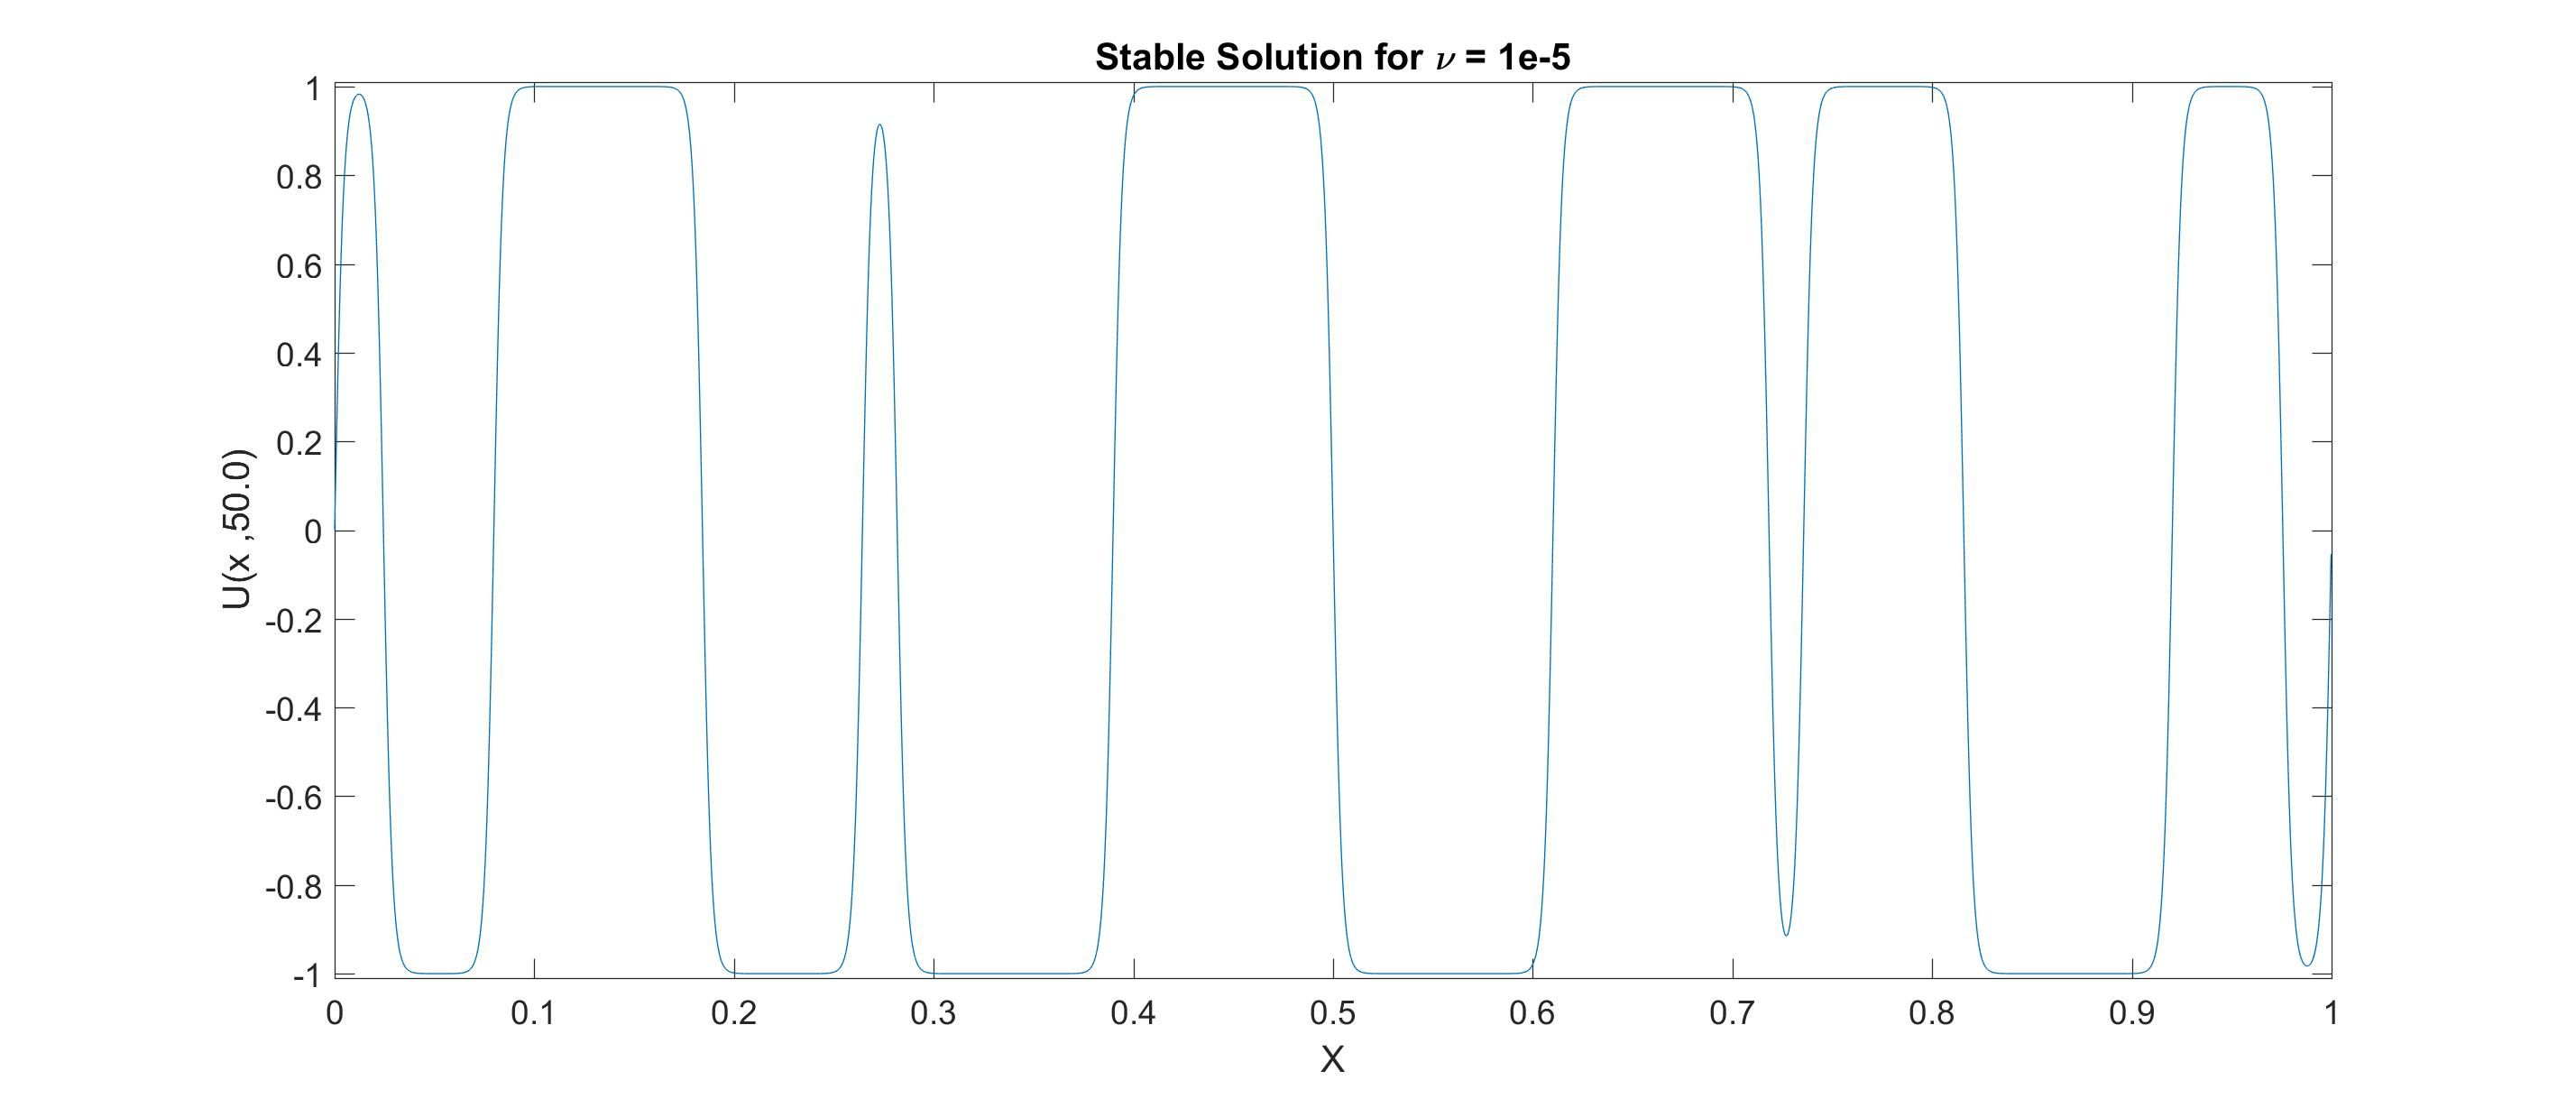
\includegraphics[scale=0.15]{Example.jpg}
	\caption{Example of a solution for Chafee-Infante equation $\alpha = 1$ $\nu=\num{1e-5}$  $N = 2^{12}=4096$, at a given time $t=50.0$ larger than the initial expansion time.}
	\label{fig:example}
%	\caption{}
\end{figure}


%In this section outline numerical scheme (eyre convex splitting theme) used and what I used this scheme for
%finding the minimum nodes
%Preliminaries section.  Put basic lemmas, theorems, and definitions here (i.e., the ones we are going to cite).
%
%Introduce Data Assimilation, the Chaffee-Infante equation, the Eyre convex splitting method
%https://www.math.utah.edu/~eyre/research/methods/papers.html 
 
 % =====================================================================
 \section{Numerical Methods}\label{secNum}
 % =====================================================================
We solve this equation on a uniform grid of $N$ points distributed uniformly on $\left[0,1\right]$ using uniform discrete time-steps of size $\Delta t = 0.01$. To ensure that initial data had a fully-resolved Fourier spectrum we used initial data in the form:
\begin{align*}
u_0(x) = \sum_{k=1}^{\frac{N}{4}}a_k\sin(2\pi kx)
\end{align*}
with $a_k$ determined randomly using a normalized Gaussian distribution. This also ensures that the solution is both periodic and satisfies homogeneous Dirichlet boundary conditions. Since the equation preserves the periodicity and oddness of the initial data.

This study uses a semi-implicit convex splitting scheme from \cite{Eyre_1997,Eyre_1998} to recover both the actual solution and the simulated data assimilation solution. Simulations have two distinct phases, an initial ramp up phase allows the actual solution to transition to a stable state, after this the actual solution and the simulated AOT algorithm solution run in tandem using a some grid configuration of h points. After a set number of time-steps, the error is measured and the second phase is repeated using a binary search algorithm to determine the minimum number of grid points of h with sufficient convergence.  


 This study uses a semi-implicit convex splitting scheme from \cite{Eyre_1997,Eyre_1998} to solve for the actual solution and the simulated data assimilation solution at every time-step. The numerical scheme we use was derived by \cite{Eyre_1997,Eyre_1998} as a stable implicit/explicit scheme:
 \begin{align*}
 {U_k}^{n+1} - {U_k}^n = dt(\nu D_{xx} + 1+2\alpha){U_k}^{n+1} + dt(-2\alpha - \alpha ({U_k}^{n})^{^2}){{U_k}^n}
 \end{align*} 
 where ${U_k}^{n} = u(x_k,t_n)$ where $dx = \frac{1}{N}$, $x_k = k dx$, $k = 0,1,2,...,N-1$,$dt = 0.01$, $t_n = n dt$. 
 %Here $x$ is discretized into $N$ points uniformly distributed on $\left[0,1\right]$ and $t$ is given in discrete time steps of size $dt$. 
 $D_{xx}$ is a centered-difference appriximation of the operator $\frac{\partial^2}{\partial x^2} $, here $\frac{\partial^2 {U_k}^{n+1}}{\partial x^2}$ is given by the second-order finite difference approximation $\frac{{U_{k-1}}^{n+1} - 2{U_{k}}^{n+1} + {U_{k+1}}^{n+1}}{dx^2} $. This results in the below system which needs to be solved at every time-step:
 \begin{align*}
 (1 - dt(\nu D_{xx} + 1+2\alpha)){U_k}^{n+1} =  (1+dt(-2\alpha - \alpha {U_k}^{n^2})){{U_k}^n}
 \end{align*}
 This method is much more stable than fully explicit methods and allows us to have a much larger time-step than other methods \cite{Eyre_1997}. In addition to this, the resulting matrix is tri-diagonal, so solving this system only has a time complexity of $O(n)$ using the Thomas algorithm.
 
 In order to apply data assimilation, we solve the following system at each time-step:
 \begin{align*}
 (1 - dt(\nu D_{xx} + 1+2\alpha)){V_k}^{n+1} =  ({V_k}^n+dt((-2\alpha{V_k}^n - \alpha {V_k}^{n^3}) +\mu(I_h(U^n) - I_h(V^n)))
 \end{align*}
 where we treat the data assimilation term explicitly. We initialize this system with ${V_k}^0 = 0$ for all $k$.
 
 Two different types of data assimilation were tested in this study with differing nodes used for the interpolation operator $I_h$. The first type was the standard uniform grid, $I_h(S)$ is the linear interpolation of $S$ over a uniform grid. The second type used a moving cluster of points which we will refer to as a sweeping probe. Data assimilation via a sweeping probe uses $M_h = M_h(t)$, where $M_h$ is the grid of $m_h$ points associated with $h$. Instead of uniformly distributing $m_h$ points, $m_h$ consecutive points are used at each time-step. \\
 $M_h{(t_n)} = \left\{x_k |~ k\in [nm \text{ (mod } N),(n+1)m_h - 1 \text{ (mod } N)] \subset\nZ \right\}$. Initially the first $m$ points are used, then at the next time-step, the next $m$ points are used. When the probe reaches the end of the domain, it periodically wraps back around to the other side.  
 
 Simulations run for this study have two distinct phases, an initial ramp up phase allows the actual solution to transition to a stable state, after this the actual solution and the simulated AOT algorithm solution run in tandem using some grid configuration of $m$ points. After a set number of time-steps, the $L^2$ norm of the difference $\norm{V-V_h}_{2}$ is used as an approximation of the error  and the second phase is repeated using a binary search algorithm to determine the minimum value of $m$ for which there is sufficient convergence. The binary search is started on the interval $\left[2,N\right]$, this interval will always contain a minimum value of $m$ as $m=N$ will always converge and the end points ($m=2$) are required nodes for the uniform grid. 
\todo{Discuss Results}

\section{Minimal Nodes for Convergence for a Static Grid}
One important result that was found through these experiments were the minimum requirements for convergence. To actually run these simulations we initialized the reference solution $u$ with randomly generated initial data and using the above numerical scheme we evolved the system overtime until it had developed into metastable structures. We then initialized the data assimilation solution $v$ with zero initial data and created a static grid $h$ consisting of $M$ uniformly distributed points. We then solved for $v$ using the data assimilation scheme with a linear interpolation of $u$ across the data assimilation nodes evaluated at the previous time step. $u$ and $v$ were then updated and $\sqrt{\Delta x}\norm{u-v}_2$ was recorded as an estimate of the error for each time-step. We allowed the system to develop to time $t_s = 50$, where $t_s$ is the time after the initial development of metastable structures. This was done because the time to develop these structures varied with the parameters $\nu$ and $\alpha$, making a uniform ending time an unfair comparison for convergence of data assimilation solutions. A binary search algorithm was used to determine the minimum value for $M$ for different values of $\nu$. It was found that for $M\propto \frac{1}{2\sqrt{\nu}}$ see \ref{fig:minimumGrid}.

While this was the case for the uniform grid, we found that the location of the data assimilation nodes were much more important than the number of nodes. We found that the only requirements for convergence were to have at least one data assimilation node in each transition layer and structure as well as the endpoints, from here on referred to as the ``optimal'' strategy for node placement. We found that if we know where the transition layers were going to form, we could achieve convergence using very few nodes. Using a posteriori knowledge of the location of the transition layers, we conducted three separate experiments. We performed data assimilation using the optimal placement strategy, the optimal placement strategy, but missing one data assimilation node in one transition layer (see \cref{fig:optimal}), and every single point on the entire domain except in the interval containing one transition layer (see \cref{fig:minimumGridFull}). It can be seen from \cref{fig:optimal,fig:minimumGridFull} and the error corresponding to them (\cref{fig:minimumGridError,fig:minimumGridErrorComplete}, respectively) that without a data assimilation node in the transition layer convergence is unobtainable, regardless of the number of nodes. 
%To show this we ran a simulation to completion and recorded the location of all the transition layers. Then, using this a postiori knowledge, we   


\begin{figure}
	\centering
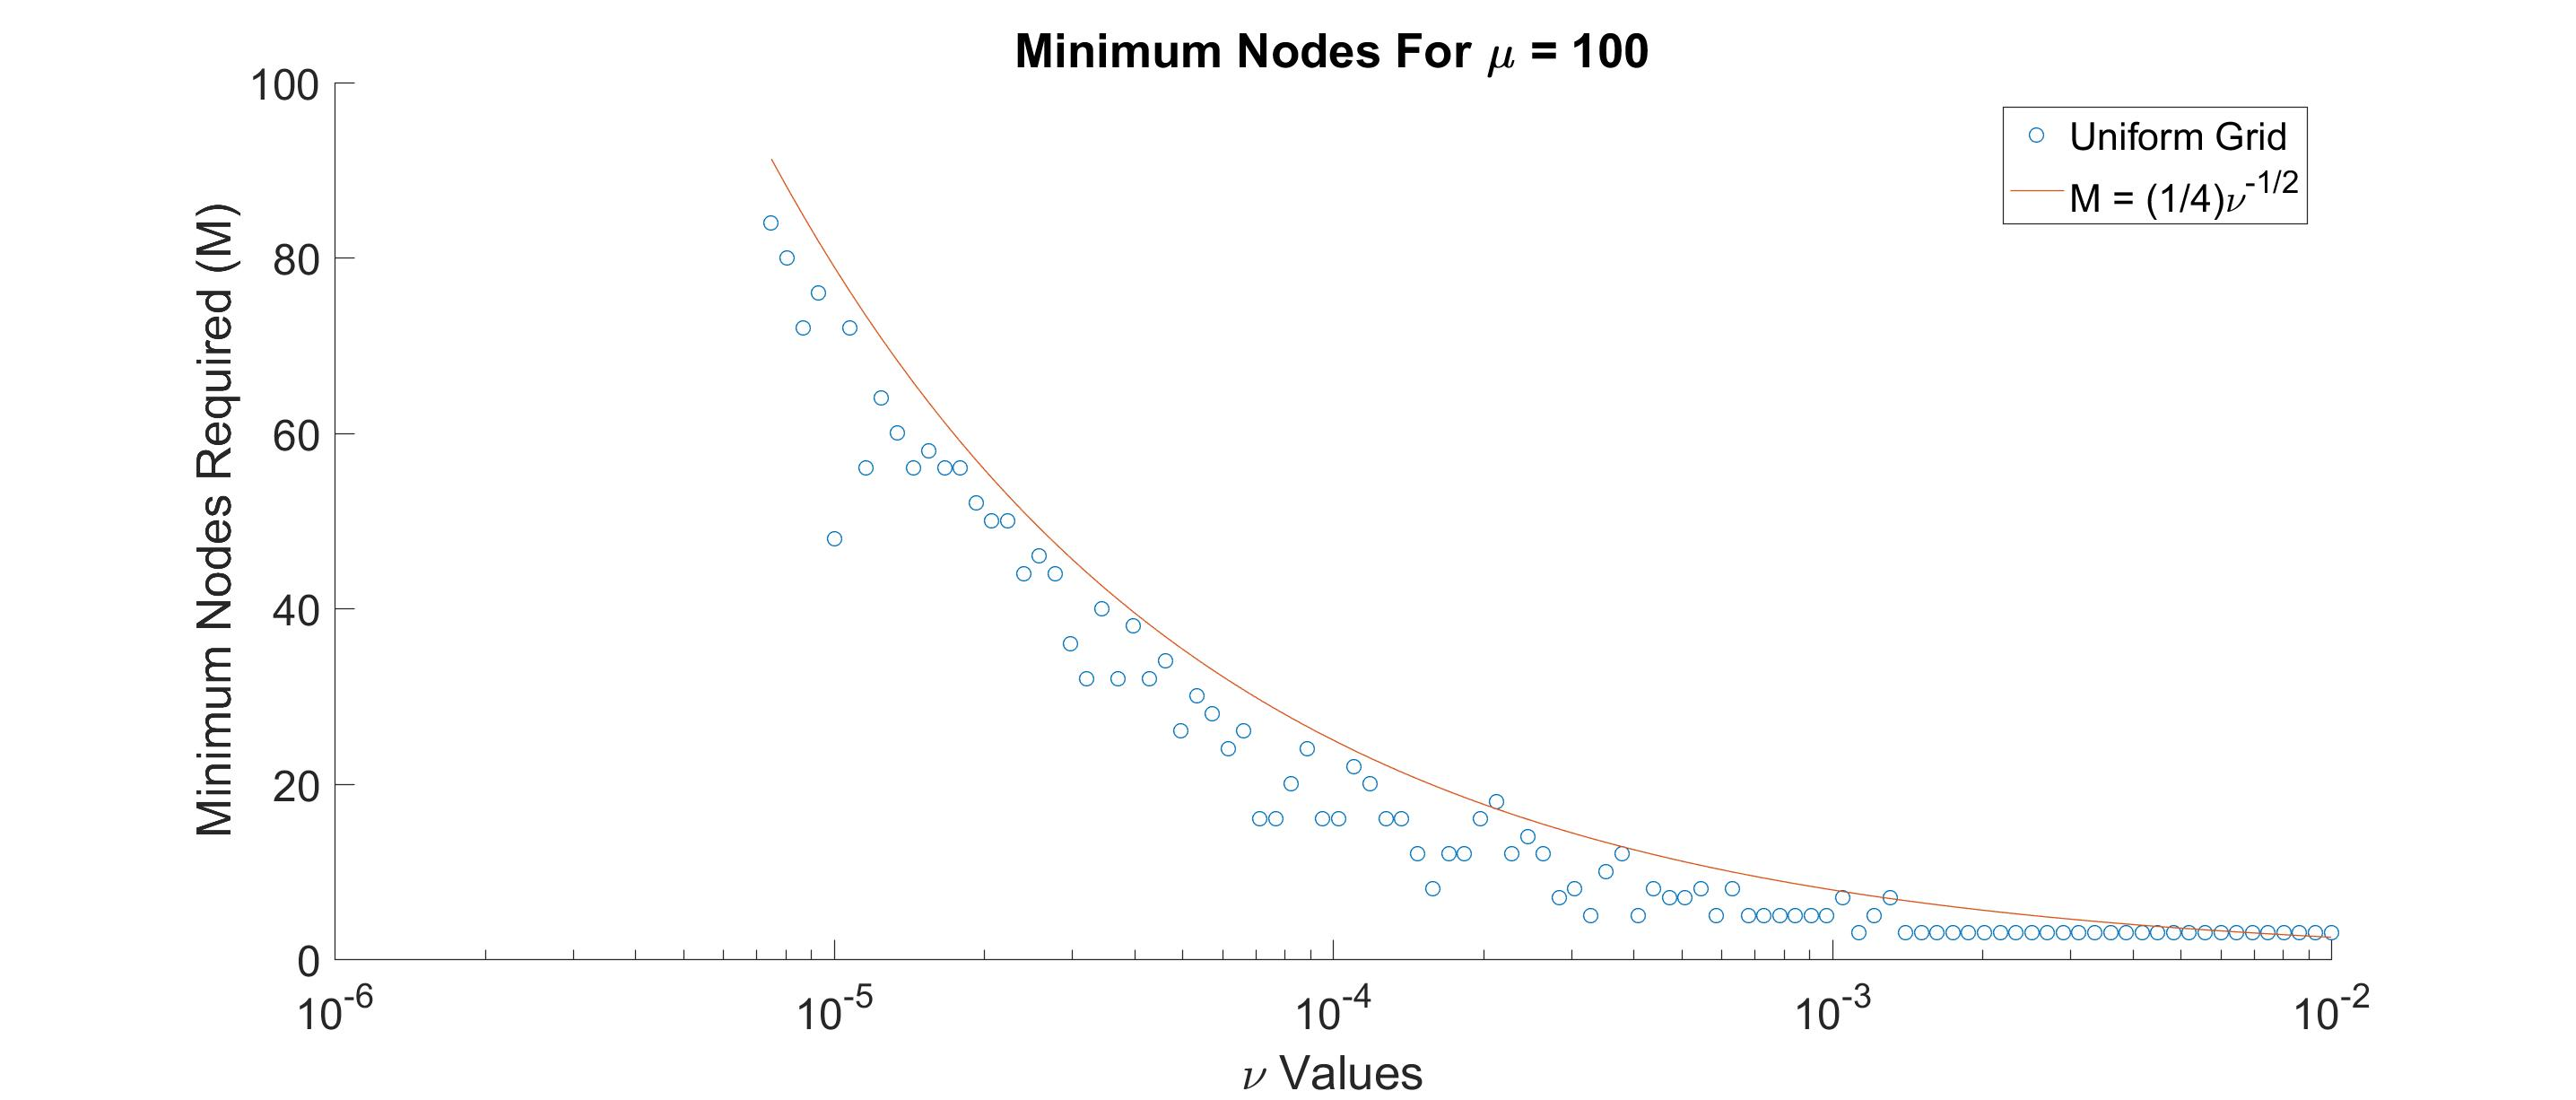
\includegraphics[scale=0.15]{MinimumNodes_Grid.jpg}
\caption{Minimum Nodes for Uniform Grid required for convergence of \num{5e-15}, $t=50$ units after ramp up period \\$\alpha = 1$ $N  =2^{12}=4096$ $\mu = 100$ }
\label{fig:minimumGrid}
\end{figure}
\begin{figure}
	\centering
	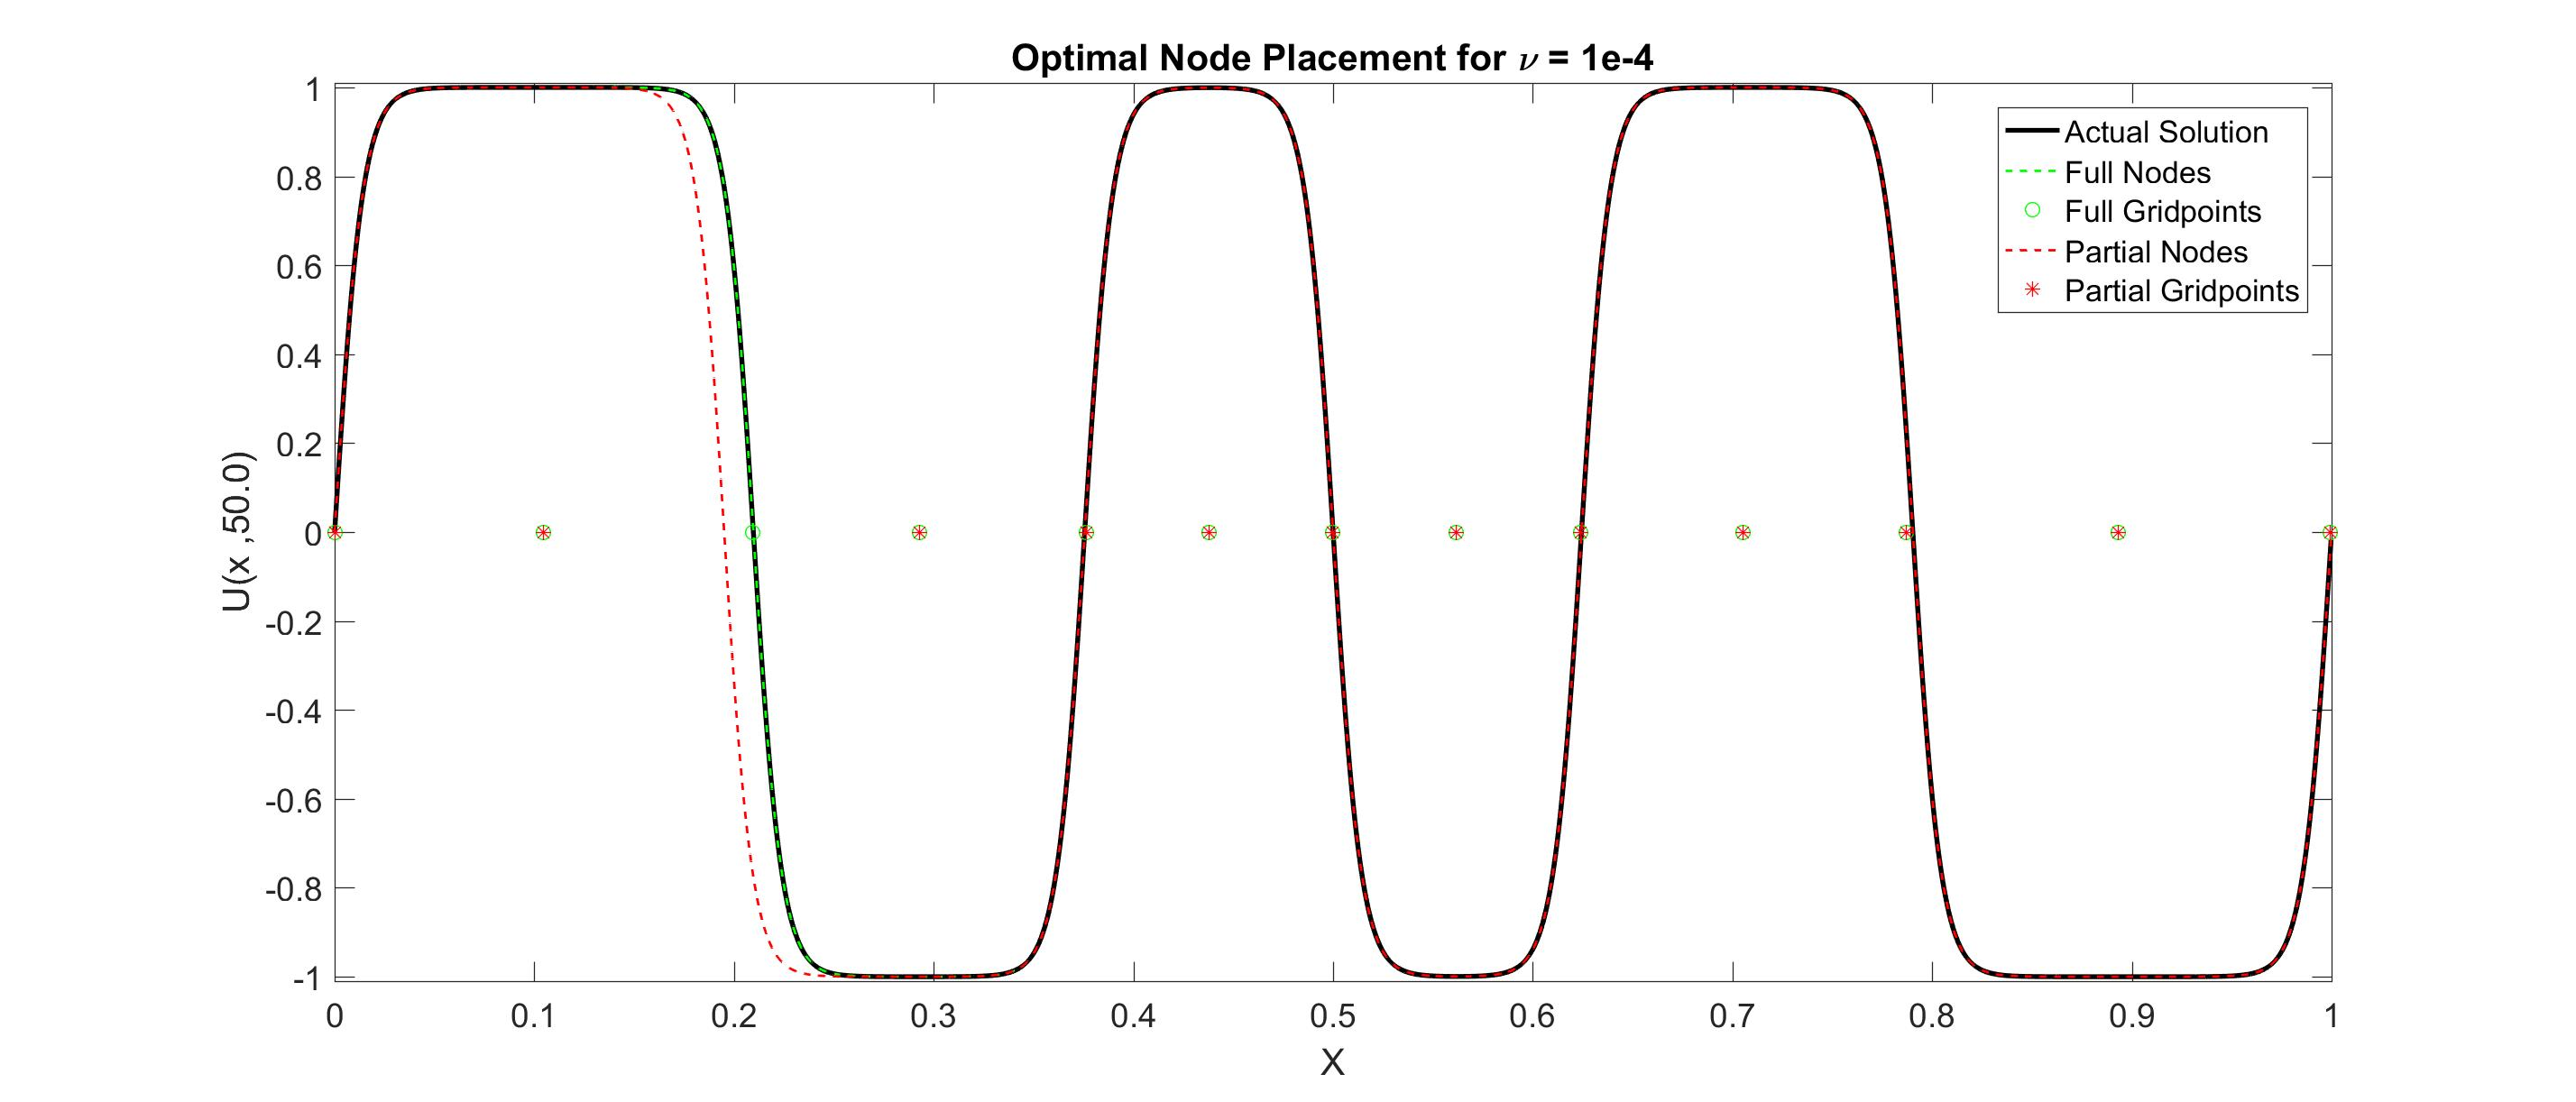
\includegraphics[scale=0.15]{Optimal.jpg}
	\caption{Data Assimilation can converge or diverge based on one grid point $\alpha = 1$ $\nu=\num{1e-4}$ $N = 2^{12}=4096$}
	\label{fig:optimal}
	%	\caption{}
\end{figure}
\begin{figure}
	\centering
	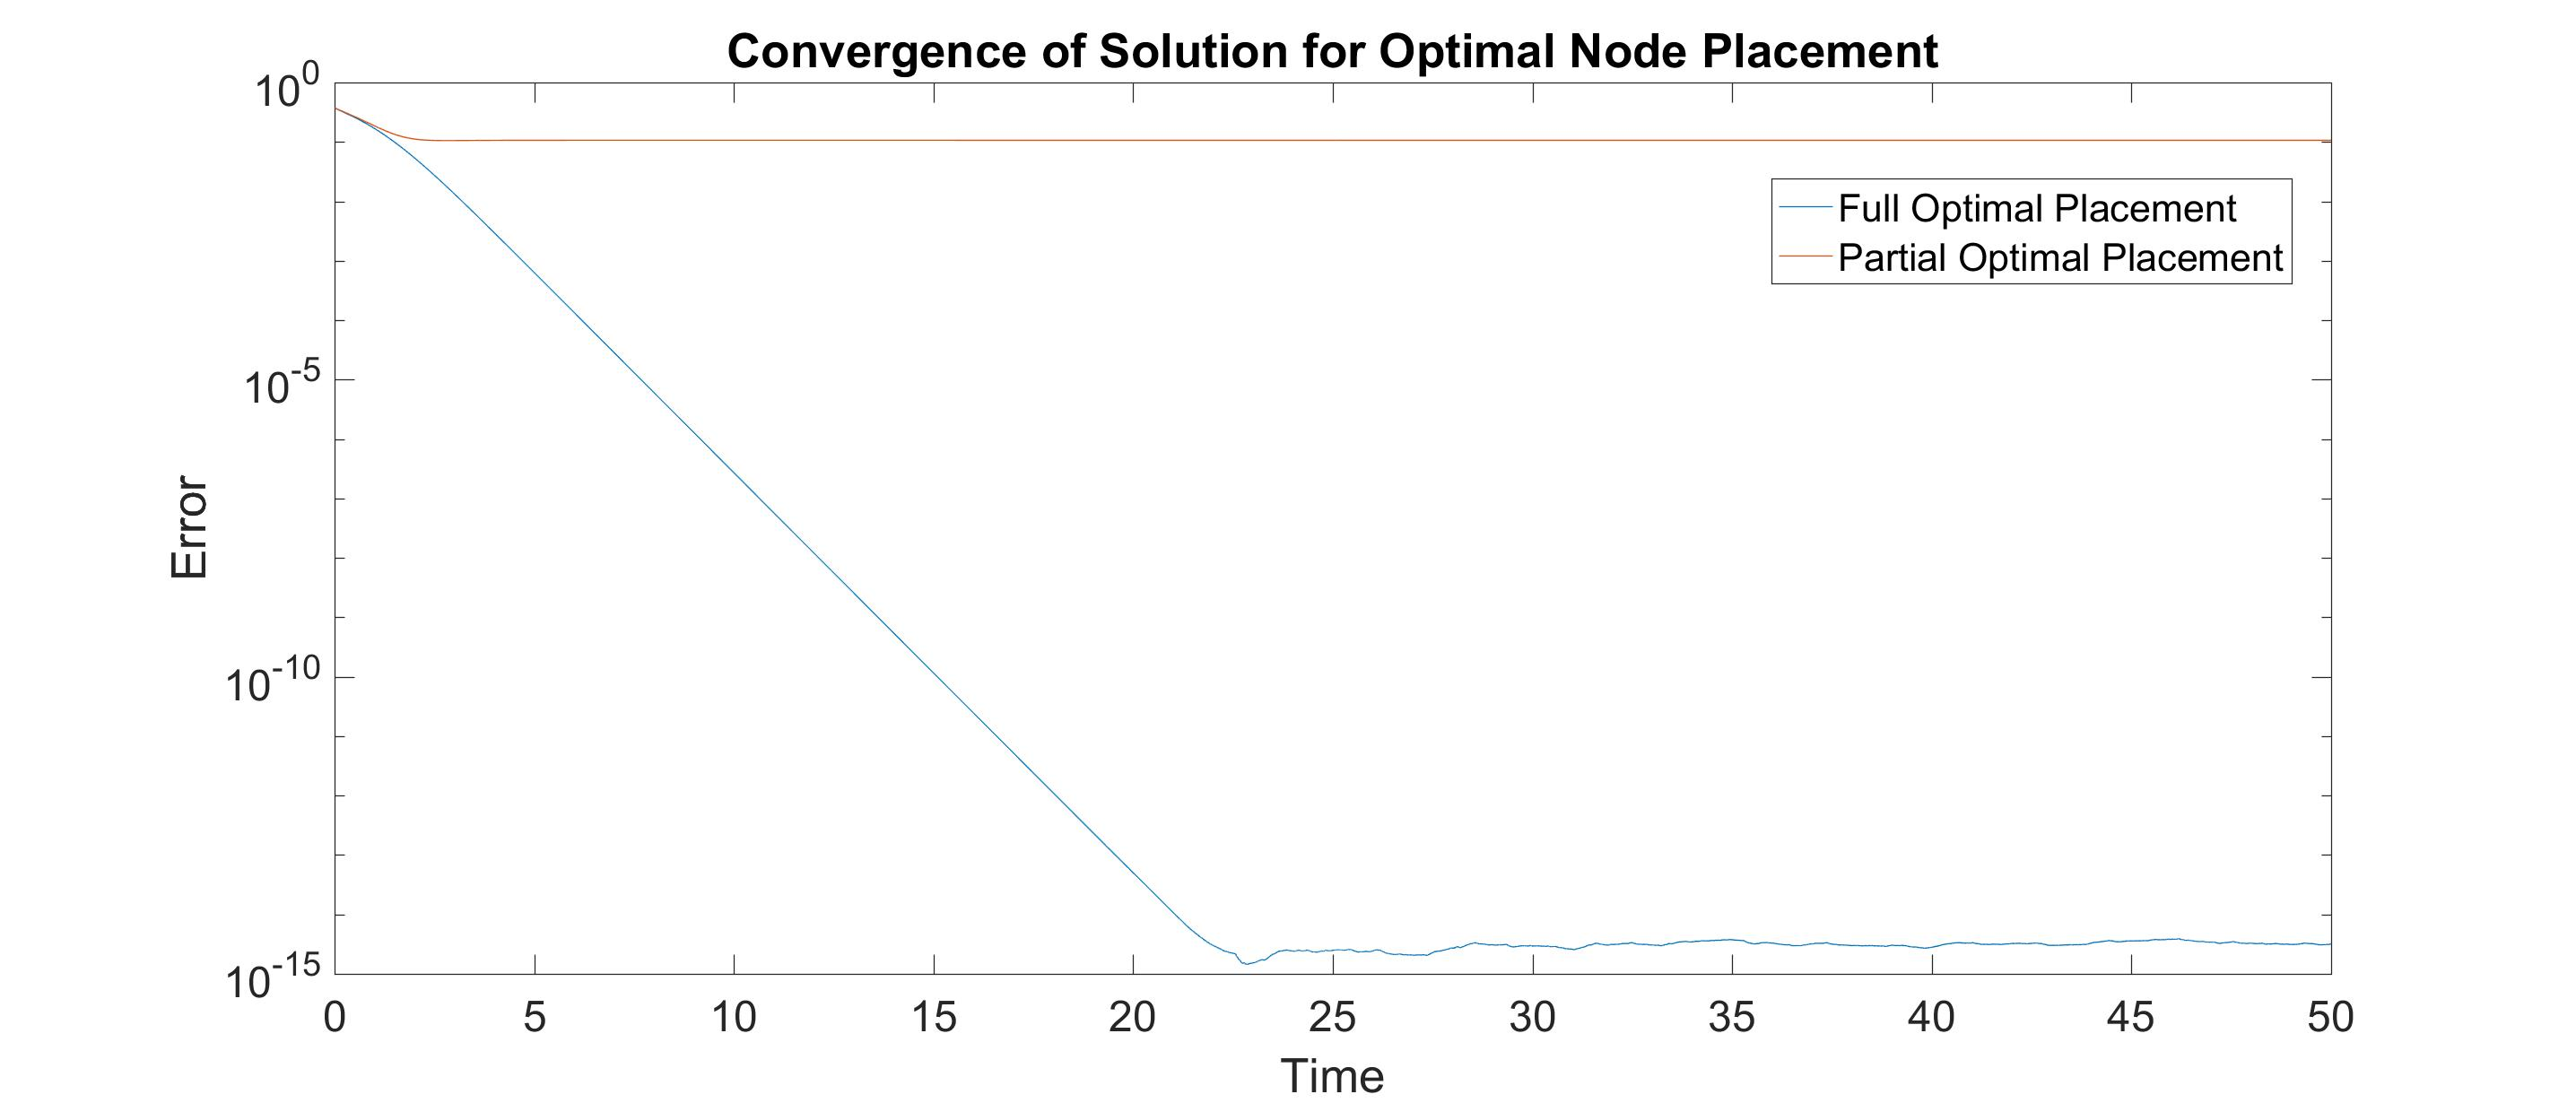
\includegraphics[scale=0.15]{Error.jpg}
	\caption{Error associated with \cref{fig:optimal} graphed over time}
	\label{fig:minimumGridError}
\end{figure}
\begin{figure}
	\centering
	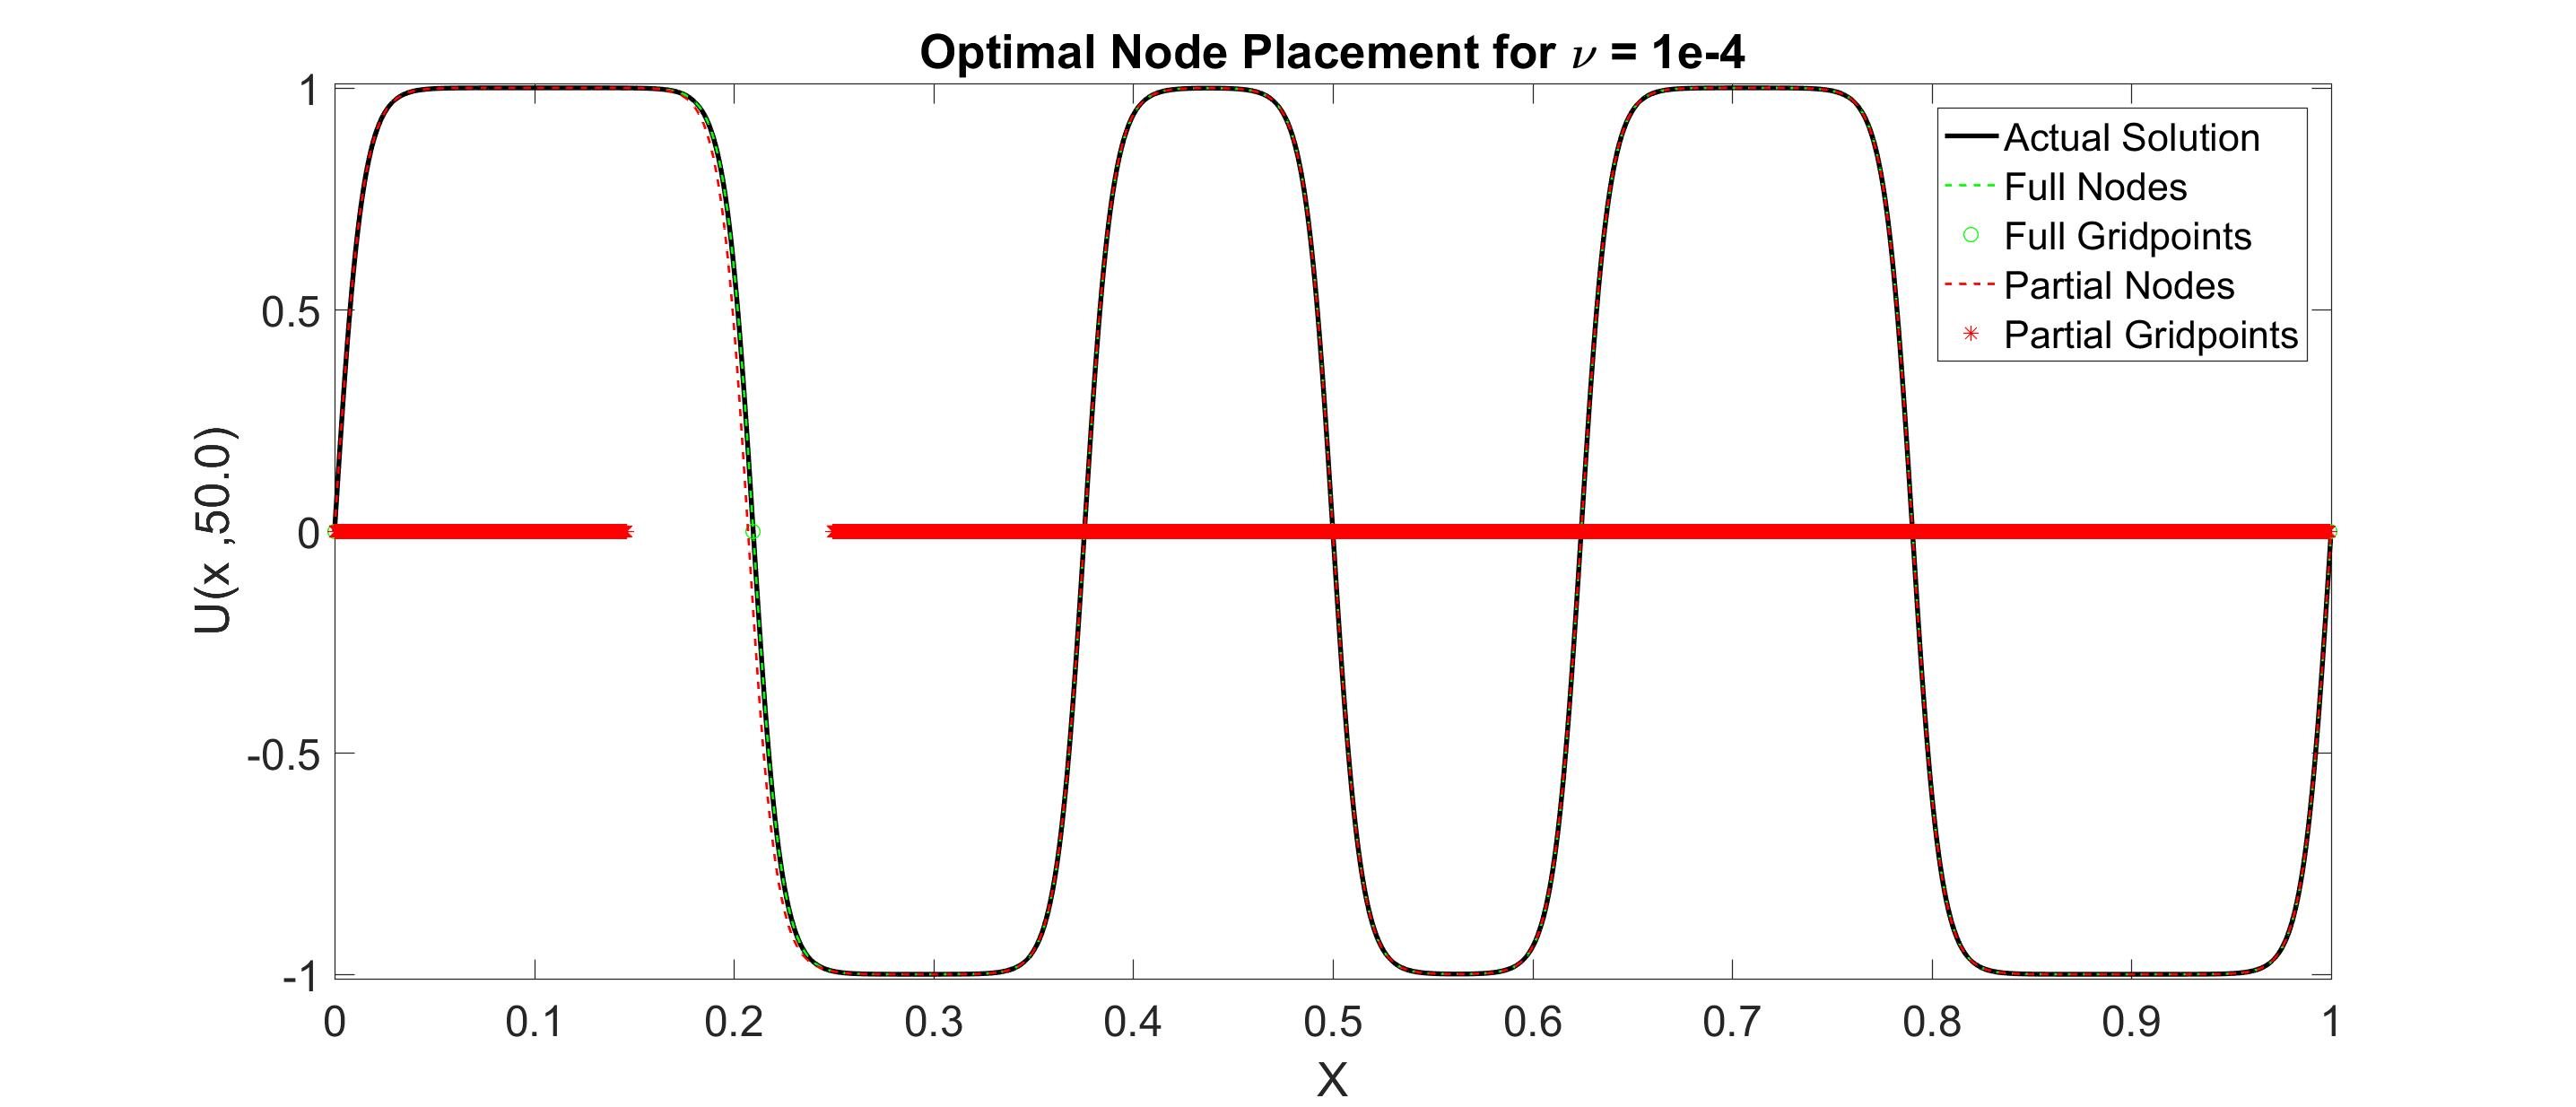
\includegraphics[scale=0.15]{CompleteOptimal.jpg}
	\caption{Data Assimilation can converge or diverge based on an interval missing not being covered $\alpha = 1$ $\nu=\num{1e-4}$ $N = 2^{12}=4096$\\NOTE: Data assimilation node placement for ``Full Nodes'' is the same as in \cref{fig:optimal}.}
	\label{fig:minimumGridFull}
\end{figure}
\begin{figure}
	\centering
	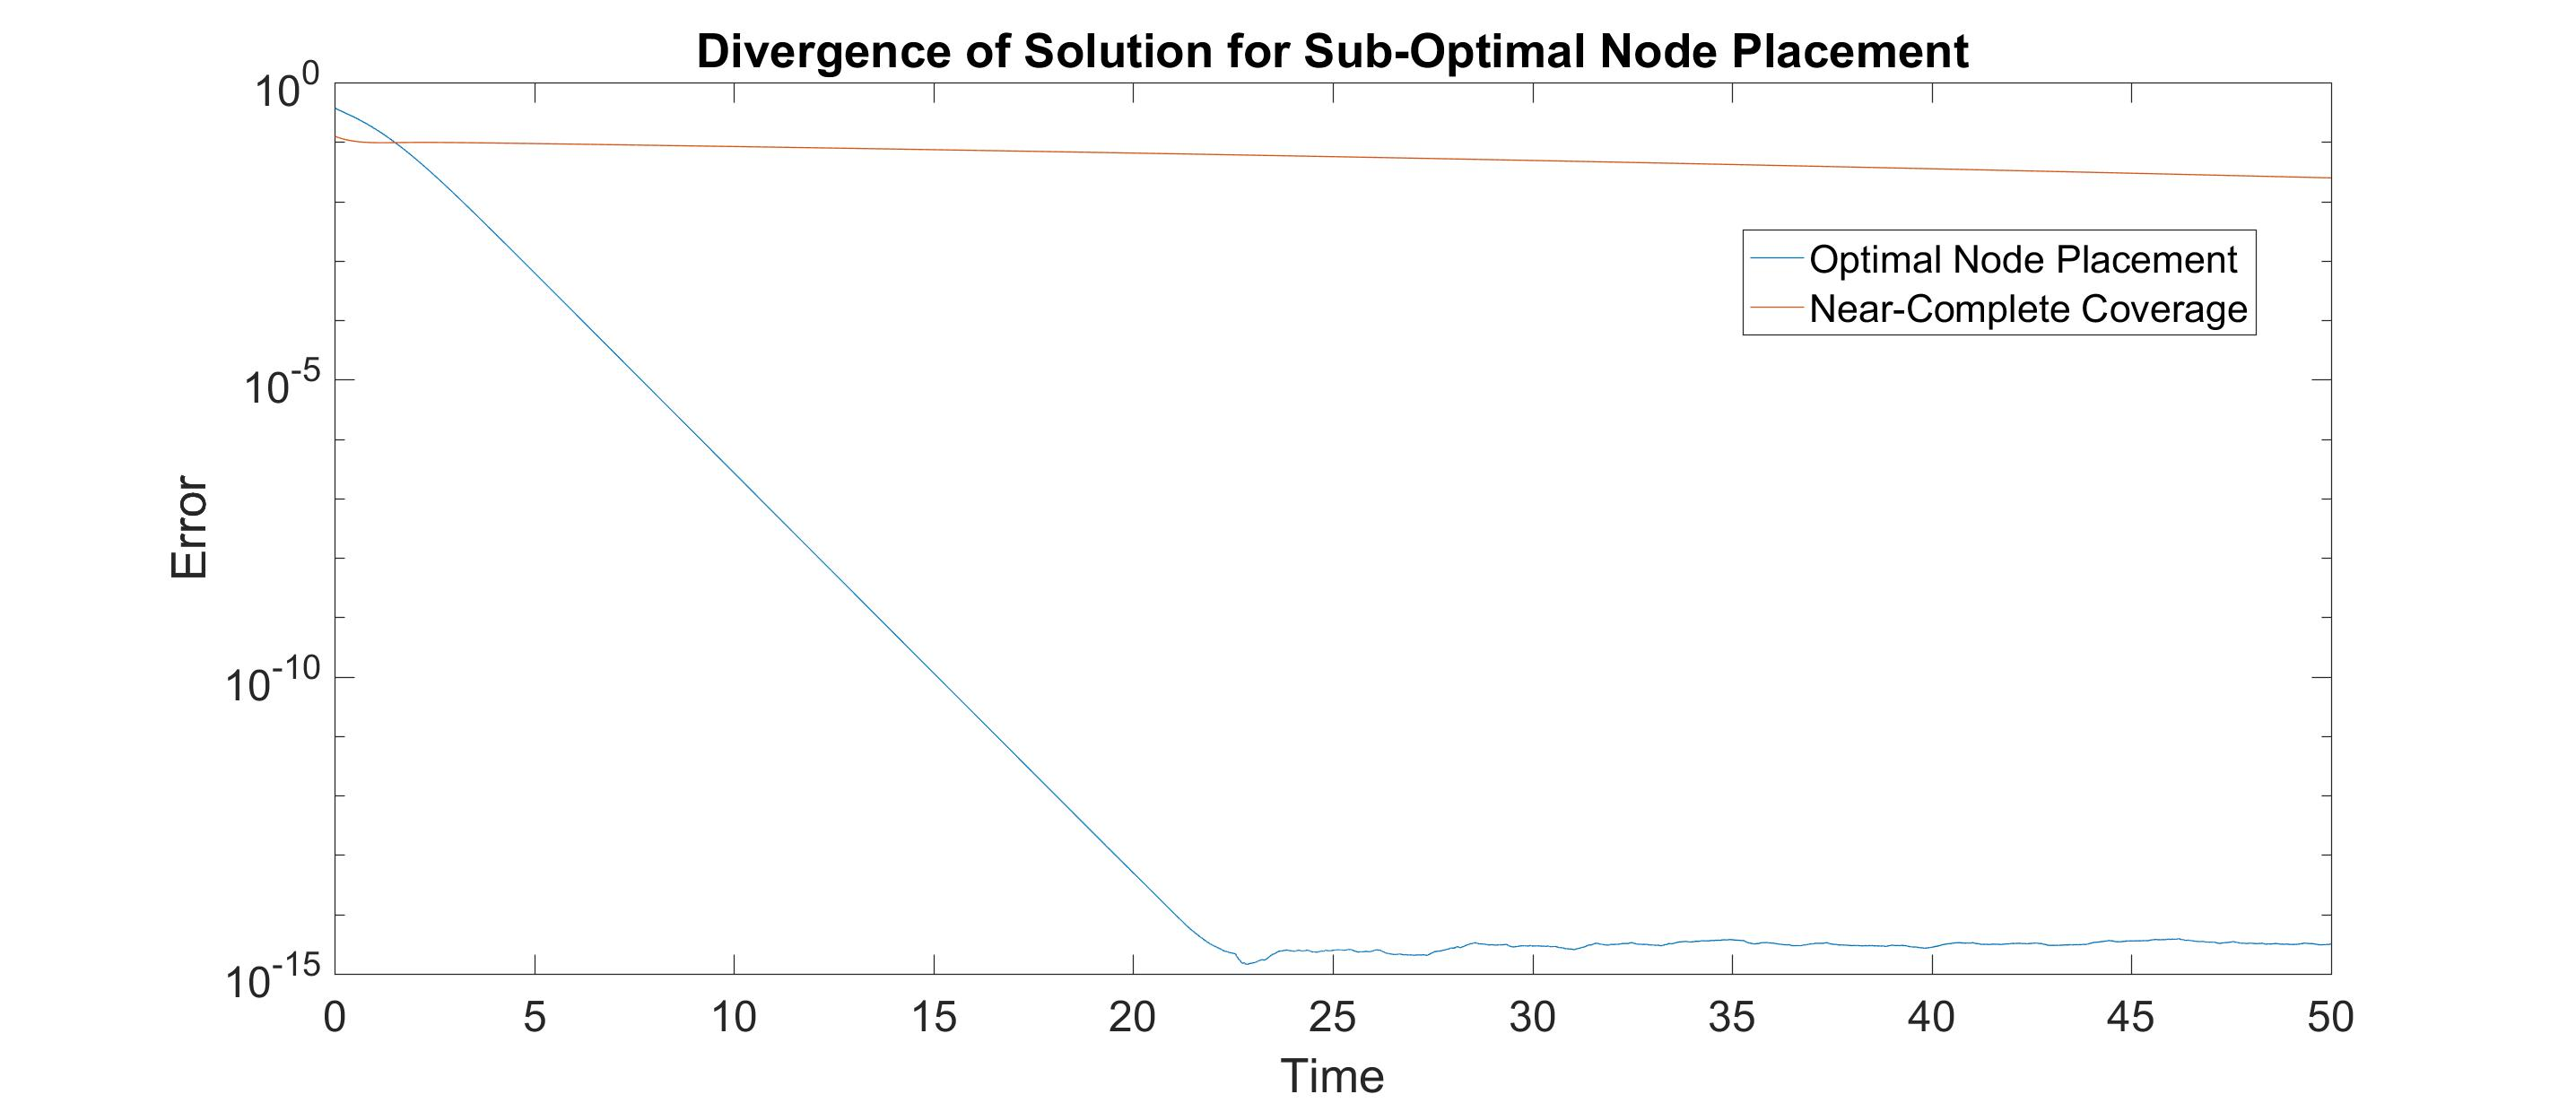
\includegraphics[scale=0.15]{CompleteError.jpg}
	\caption{Error associated with \cref{fig:minimumGridFull} graphed over time}
	\label{fig:minimumGridErrorComplete}
\end{figure}
% =====================================================================
\section{Parameter Estimation}\label{secNeat1Section}
% =====================================================================
\noindent
\todo{Search literature for formula for minimum length}
In this section detail how to find the minimum length $\lambda$ using nothing but data assimilation.

Through experimental trials we have found that the only requirement for consistent convergence to the true solution is to have at least one grid point in each transition layer and one in each structure. From the previous section we know that if a transition layer does not have a grid point, the solutions may never converge. In fact from the last section, if we knew where the transition layers were going to form, we can achieve convergence using this grid configuration. It seems that the most important parameter in determining $M$, the minimum number of nodes required for convergence, is the minimum length of the structures, $\lambda$. 


From repeated experiments we discovered that $M \propto \frac{1}{4}\nu^{-\frac{1}{2}}$ in the worst-case scenario (see \ref{fig:minimumGrid}). This was found by examining the log-log plot of $M$ vs. values of $\nu$  The worst-case scenario is a uniform distribution of the smallest possible structures across this domain. This would require the most data assimilation nodes for the optimal placement strategy, and requires the finest grid for a static uniform grid. The most nodes (using an optimal placement) will be required when all the structures have the same size $\lambda$. In this case, for there being $n_s$ structures we get $\lambda = \frac{L}{n_s} $, where $L$ is the length of the domain. We also know $M = 2n_s + 1$ or equivalently $n_s = \frac{M-1}{2}$. This can easily be shown as follows. For every structure there will be a transition layer to the right and each structure shares a transition layer with the neighboring structure except at the boundaries. Therefore, if there are $n_s$ structures, there must be $n_s - 1$ transition layers, and there are always $2$ endpoints. So, using the optimal node placement: 
\begin{align*}
M = n_s +n_s-1 +2 = 2n_s + 1
\end{align*} data assimilation nodes are required.
\begin{align*}
\lambda & = \frac{L}{n_s} \approx\frac{2L}{M} \approx\frac{8L}{\nu^{-\frac{1}{2}}} \approx 8L\sqrt{\nu}
\end{align*}

%Using only principles of data assimilation we an estimate for the inverse problem $\lambda \approx 8L\sqrt{\nu}$.
Note that in this sense, we have found an estimate for $\lambda$ in terms of $\nu$ and $L$. In this sense, we have used data assimilation to estimate the parameter $\nu$ in terms of measurements of $n_s$. We note that this may be a useful approach to solving certain inverse problems.
% =====================================================================
 \section{Sweeping Probe Data Assimilation}\label{secNeatSection}
% =====================================================================
\noindent
The main finding of this study was in the potential for sweeping probe data assimilation. In general it was found that for $\mu$ large enough for which the system is stable that for certian ranges of $\nu$ far fewer nodes are required for data assimilation via a sweeping probe (see \cref{fig:min}). To discover this, we repeated the process we used for finding the minimum number of data assimilation nodes for a uniform grid, but instead of using a uniform grid for $h$, we used a cluster of $M$ consecutive points. At each timestep we shifted every point on $h$ to the right by $M$ points. This ensures that every single point in the domain will eventually be covered, but it also limits the number of passes the probe can make of the entire system. 

The speed of the probe sounds like a limiting factor. For small $\nu$ the system tends to develop many more structures and transition layers, and thus in order to converge one would suspect that many more passes through the entire domain need to be made to capture this behavior. In practice, we found the opposite. In general, we found that even fewer data assimilation nodes are required for small $\nu$. Of course as $\nu$ grows smaller, the system develops many more structures, and contrary to our expectations, fewer data assimilation nodes were required.

Of course when $\nu$ is large it is more efficient to use a uniform grid, but there is a threshold where the methods are roughly equivalent. For $\mu =100$ this value occurs at $\nu \approx \num{2e-4}$. For smaller $\nu$ it is more effective to use the sweeping probe while for $\nu$ larger it will be more effective to use the uniform grid. Moreover the convergence of the sweeping probe is not sensitive to the number of nodes, adding extra nodes past $M$ only serve to speed up the convergence. This is not always the case for a uniform grid, as adding more points can shift the positioning of every point on the grid, meaning that convergence is not guaranteed when adding nodes. Convergence is only guaranteed for nested sets of nodes, however we found that this matters increasing little as $\nu$ decreases.


\begin{figure}
%	\missingfigure{Minimum}
	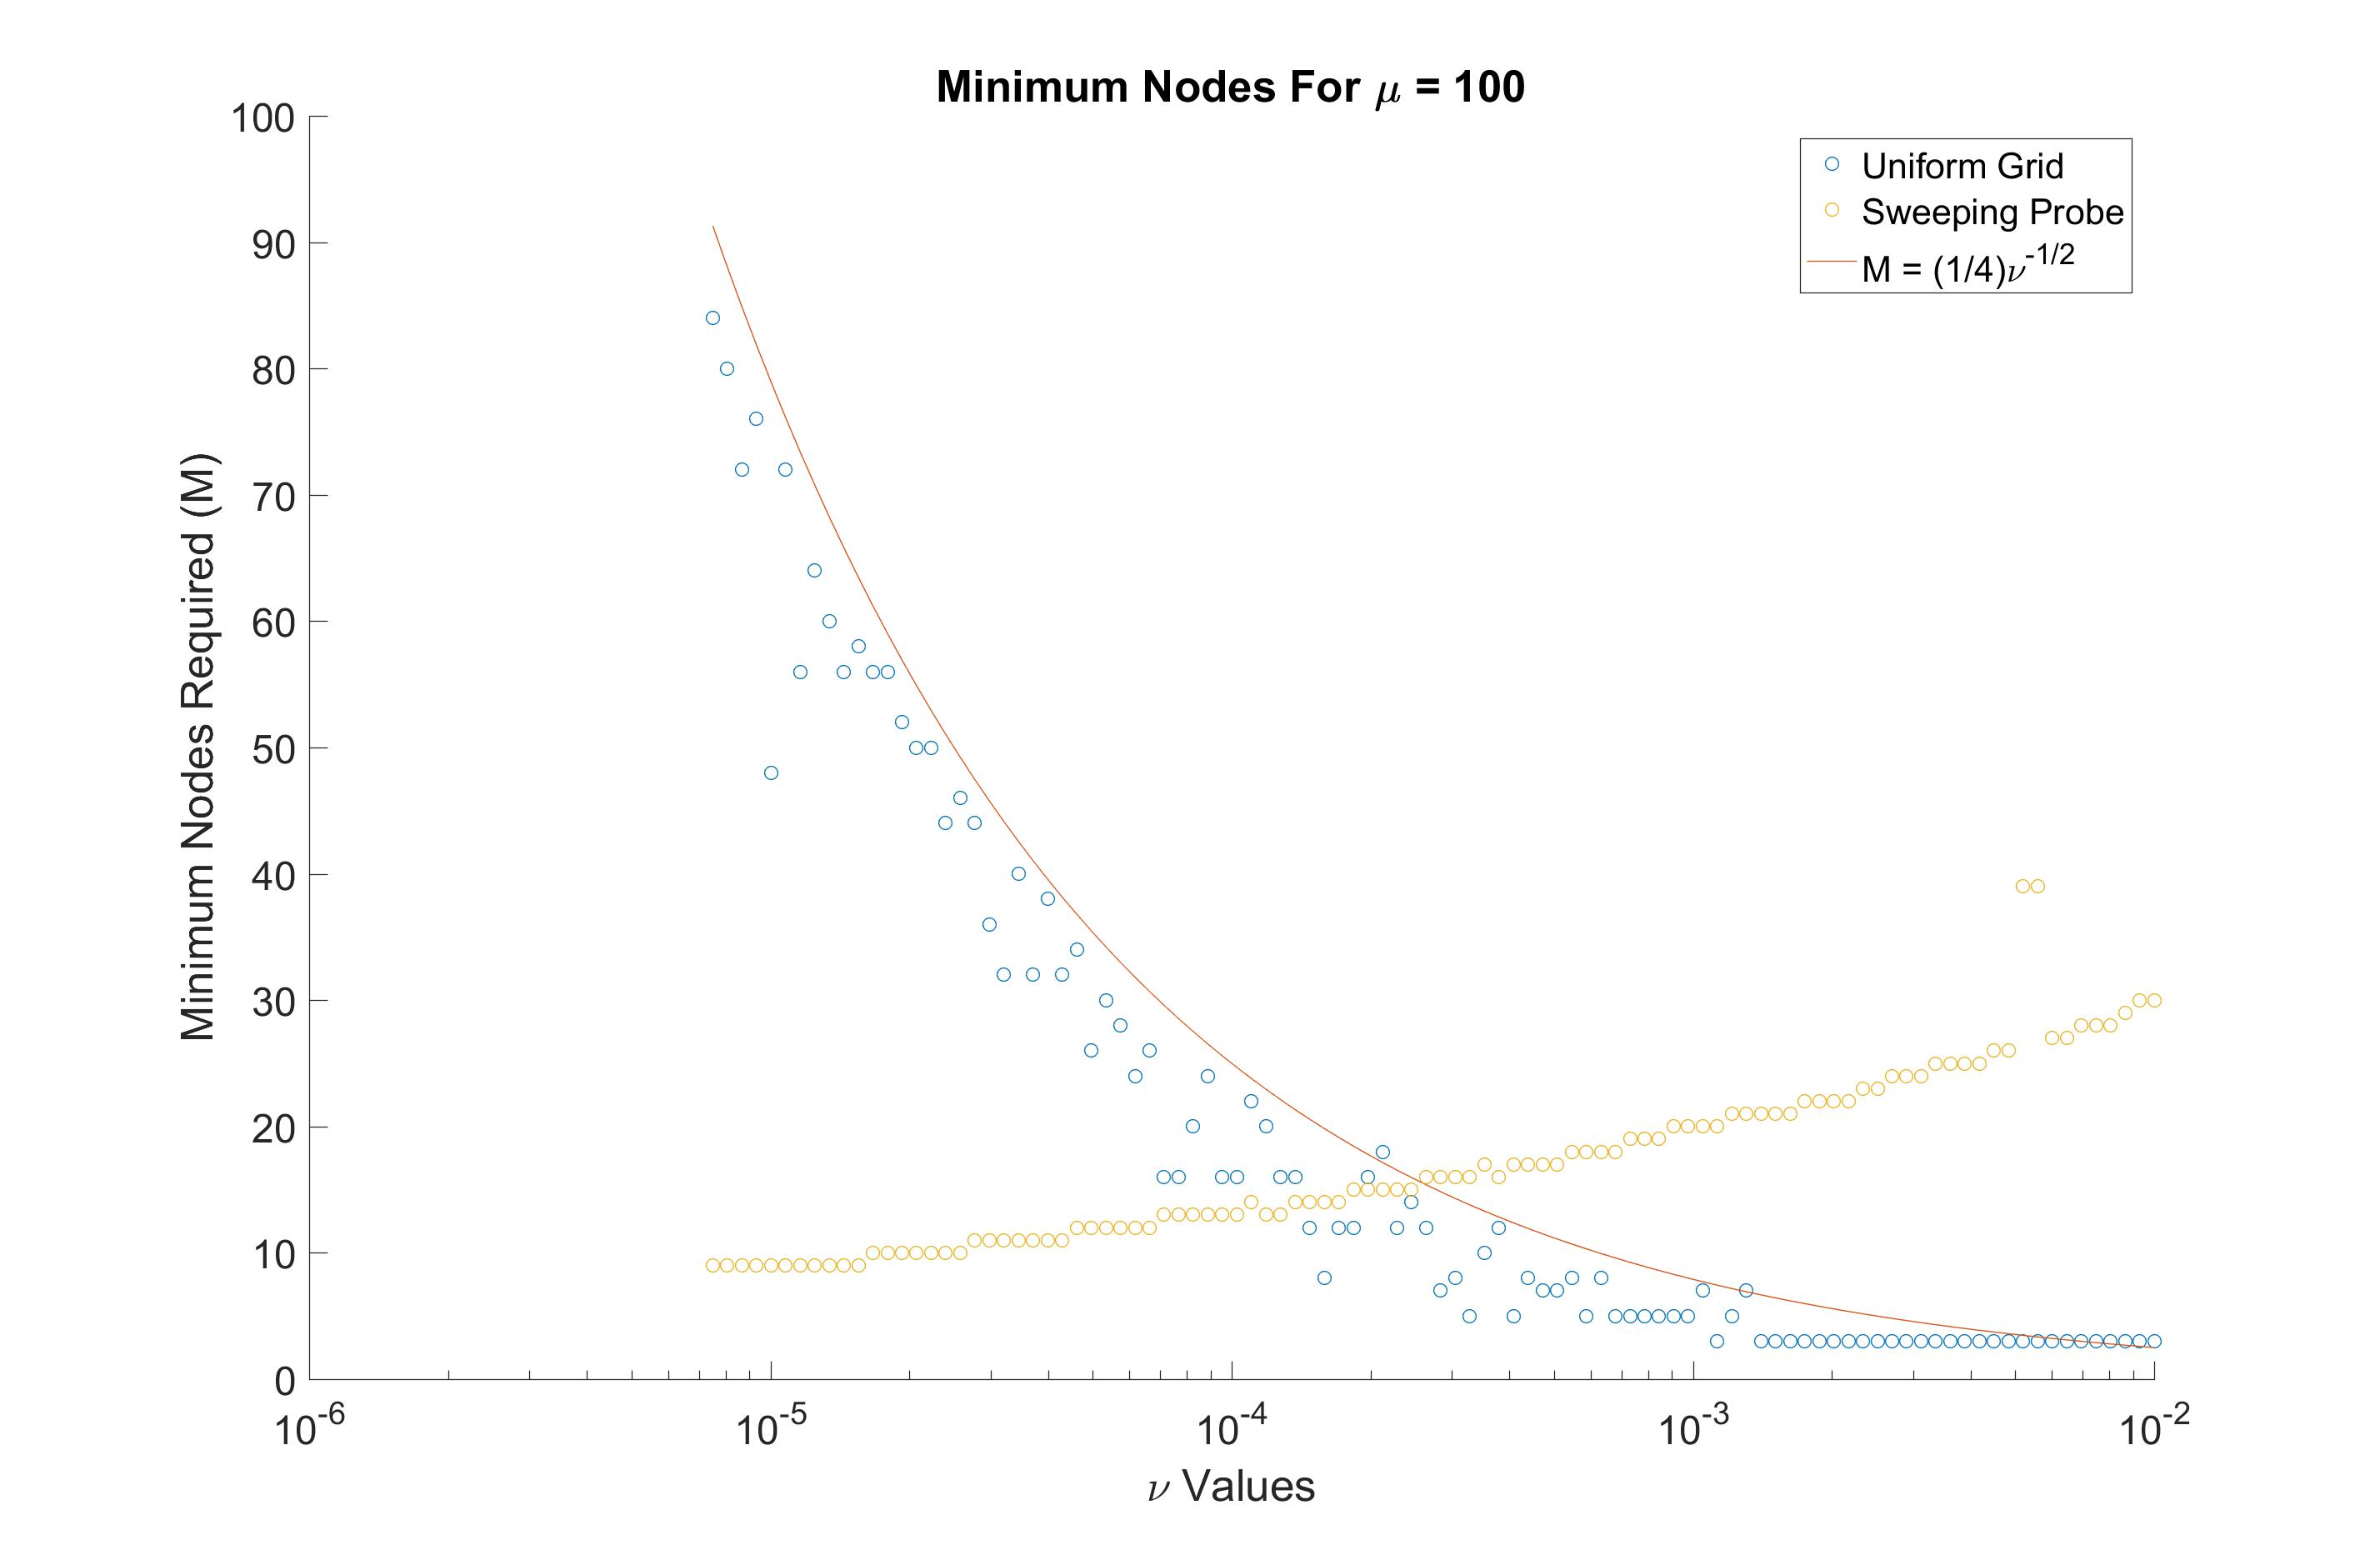
\includegraphics[scale=0.15]{Minimum}
	\caption{Minimum Nodes for Uniform Grid and Sweeping Probe required for convergence of \num{5e-15}, $t=50$ units after ramp up period \\$\alpha = 1$ $N  =2^{12} = 4096$ $\mu = 100$ }
	\label{fig:min}
\end{figure}

\section{Concluding Remarks}
This study has established sweeping probe data assimilation as a viable alternative to the uniform grid for the Chafee-Infante equation. This requires far fewer points for convergence for certain $\nu$ values and doesn't require nodes to be placed in a special configuration. More work is required to determine the viability of this type of data assimilation in higher dimensions and its usability for other equations. 
\clearpage
% \section*{Acknowledgement}
% \noindent
% This research was partially supported by grant numbers... .
% 
 %~~~~~~~~~~~~~~~~~~~~~~~~~~~~~~~~~~~~~~~~~~~~~~~~~~~~~~~~~~~~~~~~~~~~
%\begin{scriptsize}
\bibliographystyle{abbrv}%amsalpha%amsplain%plain%abbrv
%\bibliographystyle{natbib}
\bibliography{Thesis,LariosBiblio,references}
%\end{scriptsize}
%~~~~~~~~~~~~~~~~~~~~~~~~~~~~~~~~~~~~~~~~~~~~~~~~~~~~~~~~~~~~~~~~~~~~


%~~~~~~~~~~~~~~~~~~~~~~~~~~~~~~~~~~~~~~~~~~~~~~~~~~~~~~~~~~~~~~~~~~~~
\end{document}
%~~~~~~~~~~~~~~~~~~~~~~~~~~~~~~~~~~~~~~~~~~~~~~~~~~~~~~~~~~~~~~~~~~~~

